\documentclass{article}
\usepackage{inputenc,enumitem,amsmath,geometry,graphicx}
\geometry{legalpaper, portrait, margin=1in}


\title{Stanford CS224n HW A2}
\author{David Chen}
\date{August 2020}

\graphicspath{{assets/}}

\begin{document}

\maketitle

\section*{Written Questions}
\begin{enumerate}[label=(\alph*)]
    \item Since $y$ is a one-hot encoded vector, it has zeros everywhere, and 1 where $w = o$. Thus, the only non-zero term in the sum is $-y_o\log(\hat{y_o})$, which is the RHS.
    \item 
    \begin{align*}
    \boldsymbol{J}_{\text{naive-softmax}}(\mathbf{v}_c, o, \mathbf{U}) &= -\log P(O = o, C = c) \\ 
    &= -\log(\frac{\exp{(\mathbf{u}_o^\top \mathbf{v}_c})}{\sum_{w\in \text{Vocab}} \exp{(\mathbf{u}_w^\top \mathbf{v}_c})}) \\
    &= \log(\sum_{w\in \text{Vocab}} \exp(\mathbf{u}_w^\top \mathbf{v}_c)) - \mathbf{u}_o^\top \mathbf{v}_c
    \end{align*}
    We have $\frac{\partial}{\partial \mathbf{v}_c} \mathbf{u}_o^\top \mathbf{v}_c = \mathbf{u}_o$, where we take the transpose of $\mathbf{u}_o^\top$ to keep the same shape as $\mathbf{v}_c$. The derivative of the left side is as follows:
    \begin{align*}
        \frac{\partial}{\partial \mathbf{v}_c} \log(\sum_{w \in \text{Vocab}} \exp(\mathbf{u}_w^\top \mathbf{v}_c))
        &= \frac{1}{\sum_{w \in \text{Vocab}} \exp(\mathbf{u}_w^\top \mathbf{v}_c)} \sum_{x \in \text{Vocab}} \frac{\partial}{\partial \mathbf{v}_c} \exp(\mathbf{u}_x^\top \mathbf{v}_c) \\ &= \frac{\sum_{x \in \text{Vocab}} \exp(\mathbf{u}_x^\top \mathbf{v}_c) \mathbf{u}_x}{\sum_{w \in \text{Vocab}} \exp(\mathbf{u}_w^\top \mathbf{v}_c)} \\
        &= \sum_{x \in \text{Vocab}} P(O = x, C = c) \mathbf{u}_x
    \end{align*}
    Therefore,
    \[
    \frac{\partial \boldsymbol{J}_{\text{naive-softmax}} (\mathbf{v}_c, o, \mathbf{U})}{\partial \mathbf{v}_c}
    = (\sum_{x \in \text{Vocab}} \mathbf{\hat{y}_x\mathbf{u}_x}) - \mathbf{u}_o
    \]
    This can be interpreted as a difference of (expected - actual).
    
    
    Let $\theta = U^\top \mathbf{v}_c$, and let the prediction function be $\hat{y} = softmax(\theta)$
    \[
    \frac{\partial J}{\partial \theta} = (\hat{y} - y)^\top
    \]
    \begin{align*}
        \frac{\partial J}{\partial \mathbf{v}_c} &= \frac{\partial J}{\partial \theta}\frac{\partial \theta}{\partial \mathbf{v}_c}
        \\ &= (\hat{y} - y)^\top \frac{\partial U^\top \mathbf{v}_c}{\partial \mathbf{v}_c}
        \\ &= U(\hat{y} - y)^\top
    \end{align*}
    
    \item
    Again, let $\theta = U^\top \mathbf{v}_c$, and let the prediction function be $\hat{y} = softmax(\theta)$
    \begin{align*}
    \frac{\partial J}{\partial U} &= \frac{\partial J}{\partial \theta}\frac{\partial \theta}{\partial U}
    \\ &= (\hat{y} - y)\frac{\partial U^\top \mathbf{v}_c}{\partial U}
    \\ &= (\hat{y} - y)\mathbf{v}_c
    \end{align*}
    Therefore, $\frac{\partial J}{\partial \mathbf{u}_w}$ is the $w$th row of $\frac{\partial J}{\partial U}$.
    
    \item
    \[
    \sigma(x) = \frac{1}{1 + e^{-x}} = \frac{e^x}{e^x + 1}
    \]
    \[
        \frac{d\sigma(x)}{dx} = \frac{0 - (-e^{-x})}{(1 + e^{-x})^2} = \frac{e^{-x}}{1 + e^{-x}}\sigma(x) = \sigma(x)(1 - \sigma(x))
    \]
    
    \item
    Let $f(x) = -\log(\sigma(x))$.
    Then we have:
    \[
    f'(x) = \frac{\partial}{\partial x}[-\log(\sigma(x))]
    = -\frac{1}{\sigma(x)}\sigma(x)(1-\sigma(x))
    = \sigma(x) - 1
    \]
    Let $a = \mathbf{u}_o^\top \mathbf{v}_c$ and b = $-\mathbf{u}_k^\top \mathbf{v}_c$. Then,
    \[
    J = f(a) + \sum_{k=1}^K f(b)
    \]
    Thus, $\frac{\partial J}{\partial a} = f'(a)$ and $\frac{\partial J}{\partial b} = \sum_{k=1}^K f'(b)$. Additionally, we have $\frac{\partial a}{\partial \mathbf{v}_c} = \mathbf{u}_o$ and $\frac{\partial b}{\partial \mathbf{v}_c} = -\mathbf{u}_k$.
    We can now calculate
    \[
    \frac{\partial J}{\partial \mathbf{v}_c} = \frac{\partial J}{\partial a} \frac{\partial a}{\partial \mathbf{v}_c} + \frac{\partial J}{\partial b} \frac{\partial b}{\partial \mathbf{v}_c} 
    = [\sigma(\mathbf{u}_o^\top \mathbf{v}_c) - 1]\mathbf{u}_o + \sum_{k=1}^K [1 - \sigma(-\mathbf{u}_k^\top \mathbf{v}_c)]\mathbf{u}_k
    \]
    Finally, $\frac{\partial a}{\partial \mathbf{u}_o} = \mathbf{v}_c$ and $\frac{\partial b}{\partial \mathbf{u}_k} = -\mathbf{v}_c$, so
    \begin{gather*}
    \frac{\partial J}{\partial \mathbf{u}_o}
    = \frac{\partial J}{\partial a} \frac{\partial a}{\partial \mathbf{u}_o} = [\sigma(\mathbf{u}_o^\top \mathbf{v}_c) - 1]\mathbf{v}_c
    \\
    \frac{\partial J}{\partial \mathbf{u}_k}
    = \frac{\partial J}{\partial b} \frac{\partial b}{\partial \mathbf{u}_k}
    = [1 - \sigma(\mathbf{u}_k^\top \mathbf{v}_c)]\mathbf{v}_c, \forall k \in [1, K]
    \end{gather*}
    Negative sampling loss is much more efficient that naive softmax loss because it only iterates over $K$ negative examples, instead of looping over the entire vocabulary.
    
    \item 
    \begin{gather*}
        \frac{\partial \boldsymbol{J}_\text{skip-gram}}{\partial \boldsymbol{U}}
        = \sum_{\substack{-m \leq j \leq m \\ j \neq 0}}
        \frac{\partial \boldsymbol{J}(\mathbf{v}_c, w_{t+j}, \boldsymbol{U})}{\partial \boldsymbol{U}}
        \\
        \frac{\partial \boldsymbol{J}_\text{skip-gram}}{\partial \mathbf{v}_c}
        = \sum_{\substack{-m \leq j \leq m \\ j \neq 0}}
        \frac{\partial \boldsymbol{J}(\mathbf{v}_c, w_{t+j}, \boldsymbol{U})}{\partial \boldsymbol{v}_c}
        \\
        \frac{\partial \boldsymbol{J}_\text{skip-gram}}{\partial \mathbf{v}_w} (w \neq c) = 0
    \end{gather*}
    This last gradient is $0$ since these vectors are not used to calculate the loss function, and thus have no influence on the loss.
\end{enumerate}

\section*{Code Questions}

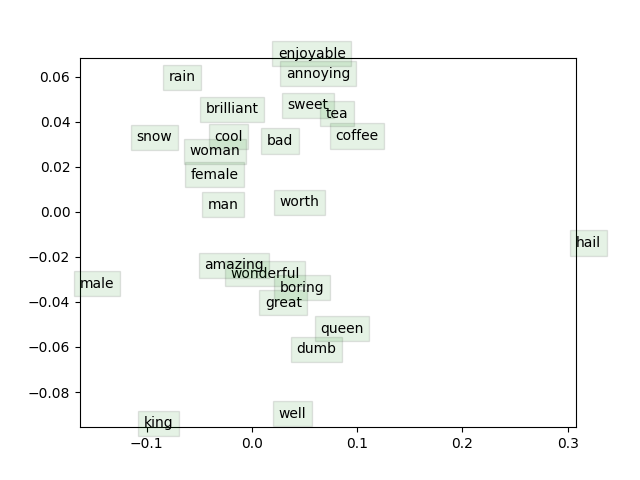
\includegraphics{word_vectors.png}

At first glance, it seems that this 2D visualization has destroyed a lot of spatial relationships between word vectors: for example, \emph{hail} is very far away from the similar words \emph{snow} and \emph{rain}. However, certain small clusters seem to be accurate: \emph{amazing}, \emph{wonderful}, and \emph{great} are nearby, and \emph{tea} and \emph{coffee} are close. Finally, the \emph{king} - \emph{queen} = \emph{male} - \emph{female} analogy holds.

    
\end{document}
